% =====================================================================
%  My Photo Diary — Installationsanleitung Synology v0.2
%  Zielgruppe: wer MPD auf einer Synology-NAS installiert (Admin im Alltag).
%  Inhaltsgleich mit spk/docs/installation.html (Web-Fassung, de/en);
%  diese TeX-Fassung ist deutsch (v0.1).
%  Gestaltung nach MPD_CI, Praeambel wie MPD_Benutzerhandbuch_v1_0.tex.
%  Erstellt 09.09.2026 im MPD-Repo (SPK-Chat), spk/docs/.
% =====================================================================
\documentclass[11pt,a4paper]{article}

\usepackage[T1]{fontenc}
\usepackage[utf8]{inputenc}
\usepackage[ngerman]{babel}
\usepackage[sfdefault]{carlito}
\usepackage{courier}
\usepackage{microtype}
\usepackage[table]{xcolor}
\usepackage[a4paper,top=2.0cm,bottom=2.0cm,left=2.5cm,right=2.5cm]{geometry}
\usepackage{array}
\usepackage{tabularx}
\usepackage{titlesec}
\usepackage{fancyhdr}
\usepackage{enumitem}
\usepackage{graphicx}
\usepackage[font=small,labelformat=empty,skip=4pt]{caption}
\usepackage[colorlinks=true]{hyperref}

\definecolor{mpdnavy}{HTML}{2C3E50}
\definecolor{mpdslate}{HTML}{34495E}
\definecolor{mpdblue}{HTML}{2E75B6}
\definecolor{mpdbluemid}{HTML}{4F81BD}
\definecolor{mpdgrey}{HTML}{7F8C8D}
\definecolor{mpdred}{HTML}{C0392B}
\definecolor{mpdrule}{HTML}{5B9BD5}
\definecolor{mpdgold}{HTML}{C8922A}
\definecolor{tblhead}{HTML}{D6E4F0}
\definecolor{tblalt}{HTML}{EBF3FB}
\definecolor{tblborder}{HTML}{CCCCCC}
\definecolor{tipbg}{HTML}{FBF5E8}

\hypersetup{linkcolor=mpdblue, urlcolor=mpdblue, citecolor=mpdblue,
  pdftitle={My Photo Diary — Installationsanleitung Synology v0.2},
  pdfauthor={Thomas Bugge / My Photo Diary}}

\titleformat{\section}
  {\color{mpdblue}\bfseries\fontsize{16}{20}\selectfont}
  {\thesection.}{0.5em}{}
  [{\color{mpdrule}\titlerule[0.8pt]}]
\titleformat{\subsection}
  {\color{mpdblue}\bfseries\fontsize{13}{16}\selectfont}
  {\thesubsection}{0.5em}{}

\pagestyle{fancy}\fancyhf{}
\renewcommand{\headrulewidth}{0pt}
\fancyhead[L]{\small\color{mpdgrey}My Photo Diary}
\fancyhead[R]{\small\color{mpdgrey}Installationsanleitung Synology v0.2}
\fancyfoot[L]{\small\color{mpdgrey}\itshape where your memories stay yours.}
\fancyfoot[R]{\small\color{mpdgrey}\thepage}

\let\mpdtt\texttt
\renewcommand{\texttt}[1]{\mpdtt{\textcolor{mpdred}{#1}}}

\arrayrulecolor{tblborder}
\setlength{\arrayrulewidth}{0.75pt}
\renewcommand{\arraystretch}{1.3}
\rowcolors{2}{white}{tblalt}
\newcommand{\kopf}[1]{\textbf{#1}}
\newcolumntype{L}{>{\raggedright\arraybackslash}X}
\setlength{\parindent}{0pt}
\setlength{\parskip}{4pt}

% Hinweiskasten wie .tip im Web (Gold-Balken links)
\newcommand{\tipp}[1]{%
  \par\vspace{4pt}\noindent
  \colorbox{tipbg}{\parbox{\dimexpr\linewidth-2\fboxsep}{%
    {\color{mpdgold}\rule[-3pt]{2pt}{1.1em}}\hspace{6pt}\parbox[t]{\dimexpr\linewidth-2\fboxsep-12pt}{#1}}}%
  \par\vspace{4pt}}

\begin{document}
\shorthandoff{"}

\begin{center}
  {\fontsize{36}{42}\selectfont\bfseries\color{mpdnavy} My Photo Diary}\\[6pt]
  {\fontsize{18}{22}\selectfont\color{mpdslate} Installation auf Synology}\\[8pt]
  {\fontsize{13}{16}\selectfont\color{mpdgrey} Version 0.2 \;·\; 2026-09-10}\\[8pt]
  {\color{mpdrule}\rule{\linewidth}{1pt}}\\[6pt]
  {\color{mpdgrey}\small Für alle, die MPD auf einer Synology-NAS einrichten \;·\;
   Danach: Benutzerhandbuch, Web-Fassung \texttt{/hilfe}}\\[6pt]
  {\color{mpdrule}\rule{\linewidth}{1pt}}\\[8pt]
  {\itshape\color{mpdnavy} „My Photo Diary — where your memories stay yours.“}
\end{center}

\vspace{1em}
\tableofcontents
\newpage

% =====================================================================
\section{Was du brauchst}

My Photo Diary läuft als Paket direkt auf deiner Synology. Du brauchst keine
Kommandozeile und musst nichts von Hand einrichten, nur diese Dinge müssen da
sein:

\begin{tabularx}{\linewidth}{|l|L|}
\hline
\rowcolor{tblhead}\kopf{Was} & \kopf{Warum} \\ \hline
Synology NAS mit \textbf{DSM 7.2} oder neuer & Ältere Versionen kennen den
  Container Manager nicht. \\ \hline
\textbf{Container Manager} (Paketzentrum) & Darin läuft My Photo Diary.
  \textbf{Bitte vorher installieren} --- DSM verlangt ihn, bevor es My Photo
  Diary annimmt. Verfügbar für die Plus-Modelle und die meisten Modelle ab
  2019, nicht für die J-Serie. \\ \hline
\textbf{Internet} während der Installation & Einmalig werden rund 150\,MB
  Grundbausteine geladen. Danach läuft alles ohne Internet; nur Landkarten
  kommen von außen. \\ \hline
Rund \textbf{1\,GB} Platz, \textbf{2\,GB} Arbeitsspeicher & Für das Programm
  und die Vorschaubilder. \\ \hline
Eine \textbf{Freigabe mit Fotos}, meist \texttt{photo} & Eure gemeinsame
  Sammlung. Sie bleibt, wo sie ist; nichts wird kopiert oder importiert. \\ \hline
\textbf{Benutzer-Home-Dienst} aktiviert & Nur nötig, wenn jede Person auch
  einen eigenen, privaten Bereich haben soll (Systemsteuerung
  \(\rightarrow\) Benutzer und Gruppen \(\rightarrow\) Erweitert). \\ \hline
\end{tabularx}

\tipp{\textbf{Was My Photo Diary nie tut:} deine Fotos verändern, verschieben
oder in eine Datenbank importieren. Ein Album ist ein Ordner, und das bleibt so.}

% =====================================================================
\section{Installation in fünf Minuten}

\begin{enumerate}[leftmargin=*, itemsep=3pt]
  \item \textbf{Container Manager installieren.} Paketzentrum \(\rightarrow\)
    suchen \(\rightarrow\) \textbf{Container Manager} \(\rightarrow\)
    Installieren. Ohne ihn nimmt DSM My Photo Diary nicht an.
  \item \textbf{Paketdatei holen.} Lade \texttt{MPD-<Version>.spk} auf deinen
    Computer.
\end{enumerate}
\begin{figure}[h]\centering
  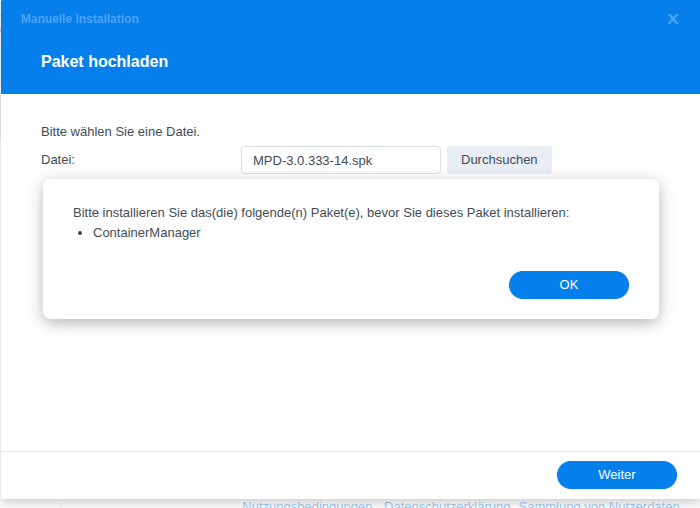
\includegraphics[width=0.82\linewidth]{screenshots/01-container-manager-fehlt.png}
  \caption{Ohne Container Manager lehnt DSM das Paket ab.}
\end{figure}
\begin{enumerate}[leftmargin=*, itemsep=3pt, start=4]
  \item \textbf{Installieren.} Paketzentrum \(\rightarrow\) \textbf{Manuelle
    Installation} \(\rightarrow\) die Datei auswählen. DSM weist darauf hin,
    dass das Paket nicht von Synology stammt: \textbf{Akzeptieren}. Fehlt der
    Container Manager, fragt DSM, ob er mitinstalliert werden soll: Ja.
  \item \textbf{Seite „Fotos“.} Wähle die Freigabe mit euren Fotos, meist
    \texttt{photo}. Die anderen Felder kannst du so lassen: Persönliche
    Bereiche liegen dann im Home-Ordner jeder Person unter \texttt{Photos}.
  \item \textbf{Seite „Erreichbarkeit“.} Der vorgeschlagene Port passt fast
    immer. Die öffentliche Adresse lässt du leer; sie ergibt sich später von
    selbst.
  \item \textbf{Seite „Benutzer“.} Du siehst die Konten deiner Synology. Gib
    jeder Person, die My Photo Diary nutzen soll, eine Rolle, und lege zwei
    Startpasswörter fest. \textbf{Mindestens ein Konto muss Admin sein}, in
    der Regel du selbst.
\end{enumerate}
\begin{figure}[h]\centering
  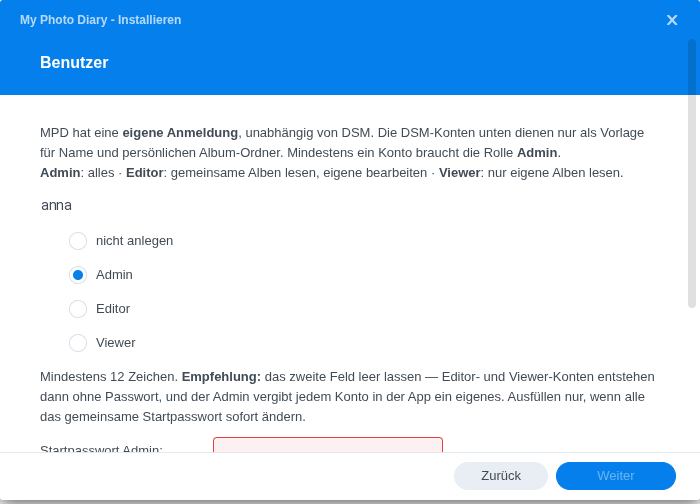
\includegraphics[width=0.82\linewidth]{screenshots/03-wizard-benutzer.png}
  \caption{Seite „Benutzer“: je Konto eine Rolle, dazu die Startpasswörter.}
\end{figure}
\begin{enumerate}[leftmargin=*, itemsep=3pt, start=8]
  \item \textbf{Fertig klicken und warten.} DSM baut jetzt das Container-Image;
    das dauert zwei bis fünf Minuten, und der Balken bewegt sich dabei kaum.
    Danach erscheint My Photo Diary im Hauptmenü.
\end{enumerate}

\begin{figure}[h]\centering
  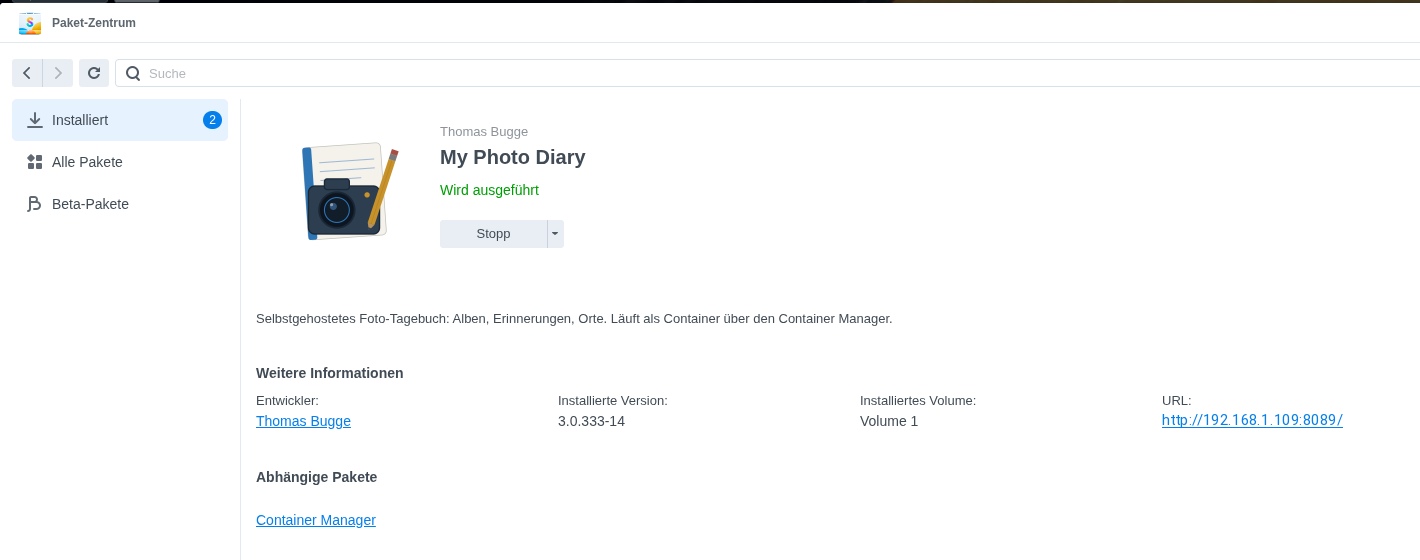
\includegraphics[width=\linewidth]{screenshots/05-paketzentrum-laeuft.png}
  \caption{Fertig: das Paketzentrum zeigt „Wird ausgeführt“ und die Adresse.}
\end{figure}

\subsection{Die drei Rollen}

\begin{tabularx}{\linewidth}{|l|L|L|}
\hline
\rowcolor{tblhead}\kopf{Rolle} & \kopf{Gemeinsame Alben} & \kopf{Eigener Bereich} \\ \hline
Admin & lesen, beitragen, gestalten & alles, dazu Benutzer und
  Einstellungen \\ \hline
Editor & lesen und beitragen (hochladen, einsortieren) & alles \\ \hline
Viewer (Betrachter) & lesen & alles \\ \hline
\end{tabularx}

\tipp{\textbf{Wichtig:} My Photo Diary hat eine \textbf{eigene Anmeldung}. Die
Synology-Konten sind nur die Vorlage für Namen und Ordner. Das
Synology-Passwort gilt hier nicht; jede Person bekommt das Startpasswort und
ersetzt es beim ersten Anmelden durch ein eigenes.}

% =====================================================================
\section{Der erste Start}

Öffne My Photo Diary über das Symbol im DSM-Hauptmenü oder direkt im Browser:
\begin{itemize}
  \item Im Heimnetz: \texttt{http://<Name-oder-IP-deiner-NAS>:8089} (oder der
    Port aus dem Assistenten)
\end{itemize}

Melde dich mit deinem Konto und dem Startpasswort an. Beim ersten Mal wirst du
gebeten, ein eigenes Passwort zu setzen. Danach siehst du eure Alben: Jeder
Ordner in der Foto-Freigabe, der Bilder enthält, ist bereits eines.

\tipp{\textbf{Geduld in der ersten Stunde:} Nach der Installation erzeugt My
Photo Diary Vorschaubilder für alle Fotos. Bei einigen tausend Bildern arbeitet
die NAS dafür bis zu einer Stunde hörbar; die App ist währenddessen schon
benutzbar, nur die Bilder erscheinen etwas langsamer.}

% =====================================================================
\section{Zugriff von unterwegs}

Im Heimnetz funktioniert alles sofort. Für den Zugriff von außen richtest du in
DSM eine Reverse-Proxy-Regel ein, ohne Cloud, verschlüsselt mit einem Zertifikat
deiner NAS:

\subsection{Eigene Domain oder Synology-Adresse}
\begin{enumerate}[leftmargin=*, itemsep=2pt]
  \item Systemsteuerung \(\rightarrow\) Anmeldeportal \(\rightarrow\)
    Erweitert \(\rightarrow\) \textbf{Reverse Proxy} \(\rightarrow\) Erstellen.
  \item Quelle: \texttt{fotos.deine-domain.de} (oder deine
    \texttt{synology.me}-Adresse), HTTPS, Port 443. Ziel: \texttt{localhost},
    HTTP, Port 8089 bzw. dein Port aus dem Assistenten.
  \item Systemsteuerung \(\rightarrow\) Sicherheit \(\rightarrow\) Zertifikat:
    ein Let's-Encrypt-Zertifikat für diese Adresse holen; DSM erneuert es selbst.
\end{enumerate}
Dazu gehören ein DNS-Eintrag für die Subdomain bei deinem Domain-Anbieter und
die Weiterleitung der Ports 80 und 443 im Router. Beides liegt außerhalb der NAS.

% =====================================================================
\section{Die App fürs Handy}

Im Browser geht alles, aber der eigentliche Alltag findet mit der
\textbf{My-Photo-Diary-App für Android} statt. Sie ist die empfohlene
Ergänzung, weil sie das kann, was ein Browser nicht kann:
\begin{itemize}
  \item \textbf{Fotos sichern:} Neue Kamerafotos wandern automatisch in den
    Durchlauf-Ordner des Jahres auf der NAS, wahlweise in die gemeinsame
    Sammlung oder in deinen privaten Bereich. Die Dateien bekommen sprechende
    Namen mit Datum und Uhrzeit.
  \item \textbf{Erinnerungen:} „Heute vor drei Jahren“ als Benachrichtigung auf
    dem Handy, direkt von deiner NAS, ohne fremden Dienst dazwischen.
  \item \textbf{Anschauen und kuratieren} unterwegs, mit Vollbild, Zeitstrahl
    und Karte.
\end{itemize}

\subsection{Einrichten}
\begin{enumerate}[leftmargin=*, itemsep=2pt]
  \item App laden und installieren: \texttt{bgg-home.de/mpd.apk}. Auf der Seite
    \texttt{bgg-home.de} steht daneben ein QR-Code auf dieselbe Adresse ---
    am Rechner öffnen, mit dem Handy scannen, laden. Android fragt dabei
    einmal, ob es Apps aus dieser Quelle installieren darf.
  \item Am Rechner im Browser bei My Photo Diary anmelden und im Menü
    \textbf{App verbinden} öffnen. Die Seite zeigt die Adresse deiner
    Installation als QR-Code.
  \item Den Code mit der \textbf{Kamera-App} deines Handys scannen --- die
    meisten Handys erkennen QR-Codes von selbst. Die Adresse antippen oder
    kopieren.
  \item In My Photo Diary beim ersten Start ins Feld \textbf{Serveradresse}
    einfügen: lange auf das Feld tippen, dann \emph{Einfügen}. Abtippen musst
    du nichts.
  \item Mit deinem My-Photo-Diary-Konto anmelden. Das ist das Konto aus dem
    Wizard, nicht das Synology-Konto.
  \item Unter „Sichern“ die Ordner wählen, die die App überwachen soll, meist
    nur den Kameraordner.
\end{enumerate}

\tipp{\textbf{Ohne App} kommen Fotos trotzdem hinein: per Datei-Station, per
Netzlaufwerk oder über einen Beisteuern-Link für Gäste. Die App macht es nur
bequem.}

% =====================================================================
\section{Updates, Daten, Deinstallation}

\subsection{Updates}
Ein Update ist eine neue \texttt{.spk}-Datei, die du wie bei der Installation
über \textbf{Manuelle Installation} einspielst. Konten, Einstellungen und
Foto-Pfade bleiben erhalten; vorher legt das Paket eine Sicherung an. Das
Update dauert wieder einige Minuten, weil das Programm neu zusammengesetzt wird.

\subsection{Wo liegen die Daten?}
\begin{tabularx}{\linewidth}{|L|L|L|}
\hline
\rowcolor{tblhead}\kopf{Was} & \kopf{Wo} & \kopf{Wert} \\ \hline
Deine Fotos und Alben & in der Foto-Freigabe und den Home-Ordnern, als ganz
  normale Ordner & \textbf{Das Einzige, was zählt.} Sichere das wie bisher. \\ \hline
Konten, Einstellungen, Standortverlauf & Freigabe \texttt{docker}, Ordner
  \texttt{MPD/data}
  & Klein, wird beim Update gesichert. \\ \hline
Vorschaubilder & ebenda, \texttt{thumb-cache} & Wegwerfbar, baut sich neu auf. \\ \hline
\end{tabularx}

\subsection{Deinstallation}
Paketzentrum \(\rightarrow\) My Photo Diary \(\rightarrow\) Deinstallieren.
Dabei werden Container, Image und der Ordner \texttt{docker/MPD/data}
entfernt, also Konten, Einstellungen und Vorschaubilder. \textbf{Deine Fotos
und Alben bleiben in jedem Fall unangetastet.} Willst du Konten und
Einstellungen behalten, kopiere den Ordner vorher weg.

% =====================================================================
\section{Wenn etwas klemmt}

\begin{itemize}
  \item \textbf{Die Installation schlägt fehl und lässt sich nicht wiederholen:}
    DSM merkt sich das Paket als „beschädigt“. Im Paketzentrum deinstallieren,
    dann erneut installieren. Hilft das nicht, liegt im Paketordner das Skript
    \texttt{tools/ds-cleanup.sh} für Administratoren.
  \item \textbf{Die Installation bricht mit einer Meldung ab:} die Meldung
    sagt, was fehlt: ein belegter Port, ein nicht gefundener Ordner, kein
    Admin-Konto. Beheben und neu starten; es bleibt nichts Halbes liegen.
  \item \textbf{Die Installation dauert sehr lange:} zwei bis fünf Minuten sind
    normal, bei langsamem Internet auch zehn. Erst danach ist etwas verkehrt;
    dann steht der Grund in \texttt{/var/packages/MPD/var/install.log}.
  \item \textbf{„Bitte installieren Sie zuerst ContainerManager“:} genau das
    --- Paketzentrum, Container Manager installieren, danach My Photo Diary
    erneut hochladen.
  \item \textbf{Das Paket lässt sich nicht starten:} läuft der Container
    Manager? Paketzentrum \(\rightarrow\) Container Manager \(\rightarrow\)
    Ausführen.
  \item \textbf{Der persönliche Bereich fehlt:} Im Home-Ordner der Person muss
    der Ordner \texttt{Photos} existieren. In der Datei-Station anlegen, dann
    im Paketzentrum einmal Stoppen und Ausführen.
  \item \textbf{Seite lädt, aber Bilder fehlen:} die Vorschaubilder entstehen
    noch (Abschnitt~3). Ein paar Minuten warten.
  \item \textbf{„Zu viele Fehlversuche“:} kurze Sperre nach mehreren falschen
    Passwörtern, eine Minute warten.
\end{itemize}

\vspace{2em}
\begin{center}
  {\color{mpdrule}\rule{0.5\linewidth}{0.8pt}}\\[6pt]
  {\color{mpdgrey}\small My Photo Diary · Installationsanleitung Synology v0.2 ·
   2026-09-09 · Web-Fassung: \texttt{installation.html}}
\end{center}

\end{document}
